\section{Struktur Navigasi}
Struktur navigasi situs web memainkan peran penting dalam meningkatkan pengalaman pengguna dengan memandu pengunjung ke informasi yang mereka cari. Menurut \citet{dewiyana2018website}, sistem navigasi yang terorganisir dengan baik sangat penting bagi pengguna untuk memahami lokasi mereka saat ini dalam situs web, mengidentifikasi langkah selanjutnya, dan mencapai tujuan mereka secara efektif. Ketika navigasi tidak konsisten atau dirancang dengan buruk, pengguna mungkin kesulitan menemukan informasi yang mereka butuhkan, sehingga menyebabkan frustrasi dan berpotensi menurunkan lalu lintas situs web.\@ \citet{dewiyana2018website} menyoroti beberapa elemen kunci yang berkontribusi terhadap navigasi yang efektif, termasuk penggunaan rambu-rambu dan alat pencari jalan. Penunjuk arah, seperti judul halaman dan logo, membantu pengguna mengorientasikan diri mereka dalam situs web, sementara strategi pencarian arah, termasuk penandaan yang jelas dan panduan lingkungan, membantu pengguna dalam menavigasi menuju konten yang mereka inginkan. Studi ini menekankan bahwa struktur navigasi yang seragam dapat mempengaruhi jumlah pengunjung situs web secara signifikan, karena meningkatkan kegunaan dan aksesibilitas.
\singlespacing{}
Lebih lanjut \citet{dewiyana2018website} mengkategorikan struktur navigasi ke dalam berbagai model, seperti model linier, hierarki, dan model spoke-and-hub. Setiap model menawarkan pendekatan berbeda dalam mengatur konten, yang dapat memengaruhi cara pengguna berinteraksi dengan situs web. Misalnya, model hierarki memungkinkan pengguna bernavigasi dari beranda utama ke subhalaman, menciptakan jalur yang jelas untuk eksplorasi. Sebaliknya, model linier menyajikan informasi secara berurutan, memandu pengguna melalui aliran yang telah ditentukan.
\singlespacing{}
Struktur navigasi merupakan komponen penting dari desain situs web yang secara langsung berdampak pada kepuasan dan keterlibatan pengguna.\@ \citet{dewiyana2018website} menegaskan bahwa dengan menerapkan strategi navigasi yang efektif, situs web dapat meningkatkan fungsionalitanya secara keseluruhan dan melayani pengunjungnya dengan lebih baik.

\subsection{Struktur Navigasi \textit{Composite}}
Struktur navigasi mengacu pada desain dan organisasi tata letak suatu situs web yang memfasilitasi eksplorasi pengguna dan pengambilan informasi. Struktur ini mencakup hubungan dan jalur antara berbagai elemen situs web, memungkinkan pengguna mengakses konten dengan efisien. Efektivitas struktur navigasi diukur berdasarkan seberapa baik struktur tersebut memungkinkan pengguna mencapai tujuan mereka, dengan indikator seperti konteks, tautan, kustomisasi, konten, dan peta situs menjadi penting dalam penilaian ini. Sistem navigasi yang terstruktur dengan baik tidak hanya meningkatkan pengalaman pengguna tetapi juga memainkan peran penting dalam menentukan kesuksesan keseluruhan situs web dengan membimbing pengguna secara lancar melalui kontennya \citep{dewiyana2018website}.

\begin{figure}[htbp]
  \centering
  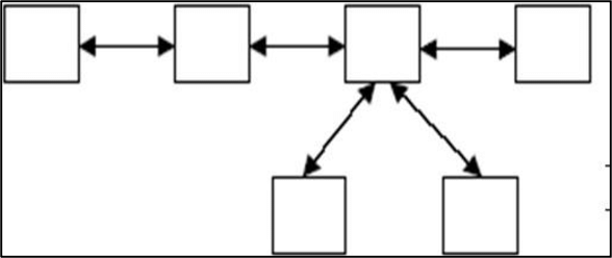
\includegraphics[width=0.85\linewidth]{images/bab-2/composite-sitemap.png}
  \caption{Struktur navigasi \emph{composite}}\label{fig:composite-sitemap}\citep{perrina2021rancang}
\end{figure}

Selain itu, pengaturan konten dan konsep dalam aplikasi web memainkan peran penting dalam menentukan struktur navigasi keseluruhan. Penataan ini memfasilitasi presentasi pola penggunaan utama bagi pengguna dan organisasi hierarkis elemen-elemen situs web, sehingga meningkatkan pengalaman navigasi yang intuitif \citep{ceci2020closed}.
